% +------------------------------------+
% |   Generated by www.docx2latex.com  |
% |   Version: 2.0.0                   |
% |  Modified by Kelley Ruehl          |
% +------------------------------------+

\documentclass[10pt,twoside]{article}
\usepackage{amsmath}
\usepackage{framed}
\usepackage{adjustbox}
\usepackage{fancyhdr}
\usepackage{float}
\usepackage[T1]{fontenc}
\usepackage{graphicx}
\usepackage[utf8]{inputenc}
\usepackage{multicol}
\usepackage{multirow}
\usepackage{txfonts}
\usepackage[svgnames]{xcolor}
\usepackage{titlesec}
\usepackage{wrapfig}
\usepackage{caption}
\usepackage{lipsum}
\usepackage[backend=biber, sorting=none]{biblatex}
\addbibresource{references.bib}
\usepackage[paperheight=27.94cm,paperwidth=21.59cm,left=2.54cm,right=2.54cm,top=2.54cm,bottom=2.54cm]{geometry}
\usepackage{hyperref}

\titleformat*{\section}{\normalsize\bfseries}
\titleformat*{\subsection}{\normalsize\bfseries}
\titleformat*{\subsubsection}{\normalsize\bfseries}
%%%%%%%%%%%%%%%%%%%%%%%%%%%%%%%%%%%%%%%%%%%%%%%%%%%%%%%%%%%%%%%%%%%%%%%%%%%%%%%%%%%%%%%%%%%%%%%%%%%%%%%%
% Header
%%%%%%%%%%%%%%%%%%%%%%%%%%%%%%%%%%%%%%%%%%%%%%%%%%%%%%%%%%%%%%%%%%%%%%%%%%%%%%%%%%%%%%%%%%%%%%%%%%%%%%%%
%\setlength\parindent{0pt}
\renewcommand{\arraystretch}{1.3}\pagestyle{fancy}
\fancyhf{}
\lhead{\thepage}
\chead{\textit{McCabe $\vert$ Proceedings of UMERC+OREC 2025}}

%%%%%%%%%%%%%%%%%%%%%%%%%%%%%%%%%%%%%%%%%%%%%%%%%%%%%%%%%%%%%%%%%%%%%%%%%%%%%%%%%%%%%%%%%%%%%%%%%%%%%%%%
% Title
%%%%%%%%%%%%%%%%%%%%%%%%%%%%%%%%%%%%%%%%%%%%%%%%%%%%%%%%%%%%%%%%%%%%%%%%%%%%%%%%%%%%%%%%%%%%%%%%%%%%%%%%
\title{WEC optimization to maximize grid economic value and avoided emissions}
\author{Overleaf}
\date{\today}

\begin{document}\thispagestyle{empty} 

\begin{center}
    \begin{figure}[h]
        \centering
        
\includegraphics[width = 0.2\textwidth]{./logo.jpg} \\
    \end{figure}
    \vspace{-\baselineskip}
    \huge
    UMERC+OREC \\
    2025 Conference \\
    \vspace{.5\baselineskip}
    \large
    \textit{12-14 August | Corvallis, OR USA} \\
    \vspace{1\baselineskip}
       
    \Large
    WEC optimization to maximize grid economic value and avoided emissions
    \vspace{.5\baselineskip}
    
    \large
    Rebecca McCabe\textsuperscript{a}\footnote{$\ast$ Corresponding author. E-mail address:  rgm222@cornell.edu \\ },
    Madison Dietrich\textsuperscript{a},
    Jiarui Yang\textsuperscript{a}, \\
    Anthony Long\textsuperscript{a},
    Khai Xin Kuan\textsuperscript{b},
    Leah Buccino\textsuperscript{a},
    Alan Liu\textsuperscript{c,d},
    Maha Haji\textsuperscript{a,e}
    
    
    \small
    \begin{center}
        \textit{\textsuperscript{a}Sibley School of Mechanical and Aerospace Engineering, Cornell University, 124 Hoy Road, Ithaca, NY 14853, USA} \\
        \textit{\textsuperscript{b}Cornell University Department of Information Science, 236 Gates Hall, Ithaca NY 14853, USA} \\
        \textit{\textsuperscript{c}Cornell University Department of Economics, 109 Tower Road, Ithaca, NY 14853, USA} \\
        \textit{\textsuperscript{d}Cornell University Department of Psychology, 116 Reservoir Ave, Ithaca, NY 14853, USA} \\
        \textit{\textsuperscript{e}Department of Systems Engineering, Cornell University, 136 Hoy Road, Ithaca, NY 14853, USA}
    \end{center}
    \normalsize
\end{center}         
\vspace{-\baselineskip}\noindent\rule{\textwidth}{0.4pt}\vspace{-\baselineskip}
%%%%%%%%%%%%%%%%%%%%%%%%%%%%%%%%%%%%%%%%%%%%%%%%%%%%%%%%%%%%%%%%%%%%%%%%%%%%%%%%%%%%%%%%%%%%%%%%%%%%%%%%
\section*{Abstract}
%%%%%%%%%%%%%%%%%%%%%%%%%%%%%%%%%%%%%%%%%%%%%%%%%%%%%%%%%%%%%%%%%%%%%%%%%%%%%%%%%%%%%%%%%%%%%%%%%%%%%%%%
Wave energy converter (WEC) design optimization has traditionally focused on minimizing the Levelized Cost of Energy (LCOE) or similar proxies.
However, this approach overlooks the reality of energy system planning, where capacity installation decisions are made to minimize total grid cost.
Grid system cost does not necessarily align with LCOE due to the complex temporal and spatial relationship between energy generation and demand.
Additionally, conventional WEC optimization neglects broader climate and electrification goals, where the reduction of lifetime equivalent CO\textsubscript{2} emissions is the key metric.
To bridge this gap, the authors previously proposed a system-level techno-economic and environmental WEC optimization framework that integrates capacity expansion modeling (CEM) and life cycle analysis (LCA) into the design objective.
This approach provides a more comprehensive assessment of wave energy's net value proposition beyond conventional cost metrics.
In this work, we implement this methodology in a new open-source multidisciplinary design optimization framework.
Our implementation leverages the GenX CEM, the PowerGenome energy data interface, the Idemat LCA dataset, and the MDOcean WEC model.
A surrogate model of the CEM reduces computation time compared to the naive CEM-in-the-loop approach.
We present preliminary optimization results for the Reference Model 3 (RM3) WEC, demonstrating the impact of optimizing for new value-driven economic and environmental system metrics compared to the standard LCOE.
For the scope of emissions controllable in the early design phase, the environmental objective aligns well with the economic one, indicating that design-for-environment techniques may not be relevant until later in the design process.
Meanwhile, the grid system economic objective is hypothesized to favor larger WECs in scenarios with winter generation deficits, such as the U.S. northeast with electrified heat loads, where the value of capturing energetic winter sea states outweighs the cost of surviving them.
On the other hand, systems with storage constraints should favor smaller WECs, where the avoided storage cost due to more consistent power generation outweighs the penalty in absorbed power.
Finally, we discuss the broader implications of these findings for future WEC design optimization priorities.
 \hfill 

\vspace{.5\baselineskip}
\textit{Keywords:} techno-economic model, environmental impact assessment, energy grid integration, multidisciplinary design optimization, life cycle analysis, capacity expansion model

\noindent\rule{\textwidth}{0.4pt}

%%%%%%%%%%%%%%%%%%%%%%%%%%%%%%%%%%%%%%%%%%%%%%%%%%%%%%%%%%%%%%%%%%%%%%%%%%%%%%%%%%%%%%%%%%%%%%%%%%%%%%%%
\section{Introduction}
%%%%%%%%%%%%%%%%%%%%%%%%%%%%%%%%%%%%%%%%%%%%%%%%%%%%%%%%%%%%%%%%%%%%%%%%%%%%%%%%%%%%%%%%%%%%%%%%%%%%%%%%
Advances in wave energy converter (WEC) multidisciplinary design optimization show the potential to reduce the Levelized Cost of Energy (LCOE) X-fold \cite{mccabe_leveraging_2025}.
However, LCOE does not fully capture the value of WECs \cite{mowers_evaluation_2021,moraski_beyond_2025}.
Alternative metrics include net present value and payback period for off-grid contexts \cite{jenne_powering_2021}, net value of energy and profitability metrics in technology-specific economic evaluation \cite{mowers_evaluation_2021,makaremi_economic_2025}, and total grid system cost and lifetime equivalent CO\textsubscript{2} emissions in energy system planning and climate change mitigation \cite{moraski_beyond_2025}.
Prior studies of WEC grid integration reveal benefits including reduced curtailment, increased capacity factor, and improved grid reliability due to seasonal complementarity with solar, proximity to coastal load, and wave resource consistency (cite WEC CEM/EDs and WEC grid value lit).
Considering energy system factors in the early design phase can steer WEC development to fully leverage this potential value and maximize climate benefit.

Recent studies for other technologies incorporate linearized design considerations into energy system optimization \cite{schwartz_value_2023,ricks_value_2022}, energy system considerations into design optimization \cite{mehta_designing_2024}, and combined energy system and environmental considerations into design optimization \cite{canet_eco-conscious_2023,kainz_technological_2024}.
This study is the first to apply integrated design and energy system optimization to WECs, and also a methodological improvement over similar studies for other technologies. 
Specifically, a surrogate capacity expansion model within a nonlinear design optimization more fully captures design-grid coupling while maintaining computational efficiency, a technique which the authors conceptually introduce in \cite{mccabe_system_2023} and here implement via dynamic system parameterization.
   % -  prior work showing that CEM is more important than economic dispatch?

\section{Methodology}
\subsection{Optimization problem formulation}
The WEC to be optimized is the Reference Model 3 (RM3) \cite{neary_reference_2014}, a two-body heaving point absorber.
We utilize MDOcean \cite{mccabe_mdocean_2024}, an open-source WEC multidisciplinary design optimization framework, with the same design variables and constraints as \cite{mccabe_leveraging_2025}.
The twelve design variables include five bulk geometric dimensions (float and spar diameter and height, and clearance between the float tubes and spar), two generator ratings (maximum power and maximum force), and five structural dimensions (float, spar, and damping plate material thicknesses, and float and damping plate stiffener heights).
See \cite{mccabe_leveraging_2025} for variable ranges and rationales.
Constraints create substantial nonconvexity and include pitch stability, hydrostatic balance, structural survival, and dynamic amplitude limits.
New in this study, the primary optimization objective is the grid cost CEM output, but when the WEC is not economically viable, the objective becomes the margin to viability to avoid flatness.
For multi-objective optimization, a second new objective of net eco-value per unit energy captures system-level environmental impacts.
MDOcean utilizes gradient-based nonlinear programming for single-objective optimization and combines gradient-based and gradient-free methods for multi-objective optimization \cite{mccabe_leveraging_2025}.
\figureautorefname~\ref{fig:n2} depicts the optimization structure via an xDSM diagram \cite{lambe_extensions_2012}, with design variables on the top row and objectives and constraints in the rightmost two columns.

\subsection{Modeling}
MDOcean integrates hydrodynamic, structural, control, and economic models, which \cite{mccabe_leveraging_2025} details.
%The model handles nonlinear dynamics including drag and generator force limits.
This study introduces new modules for ``grid'' and ``environment'' to MDOcean. The middle of \figureautorefname~\ref{fig:n2} depicts simulation connections to integrate the modules.
As \cite{mccabe_system_2023} proposes, CEM optimizations are performed ahead of the design optimization for a wide set of inputs that reflect the range of possible WEC designs and world scenarios. The grid module of the design optimization captures CEM results in a surrogate model to reduce computation time.
\begin{wrapfigure}[31]{r}{0.76\textwidth}
    \centering
    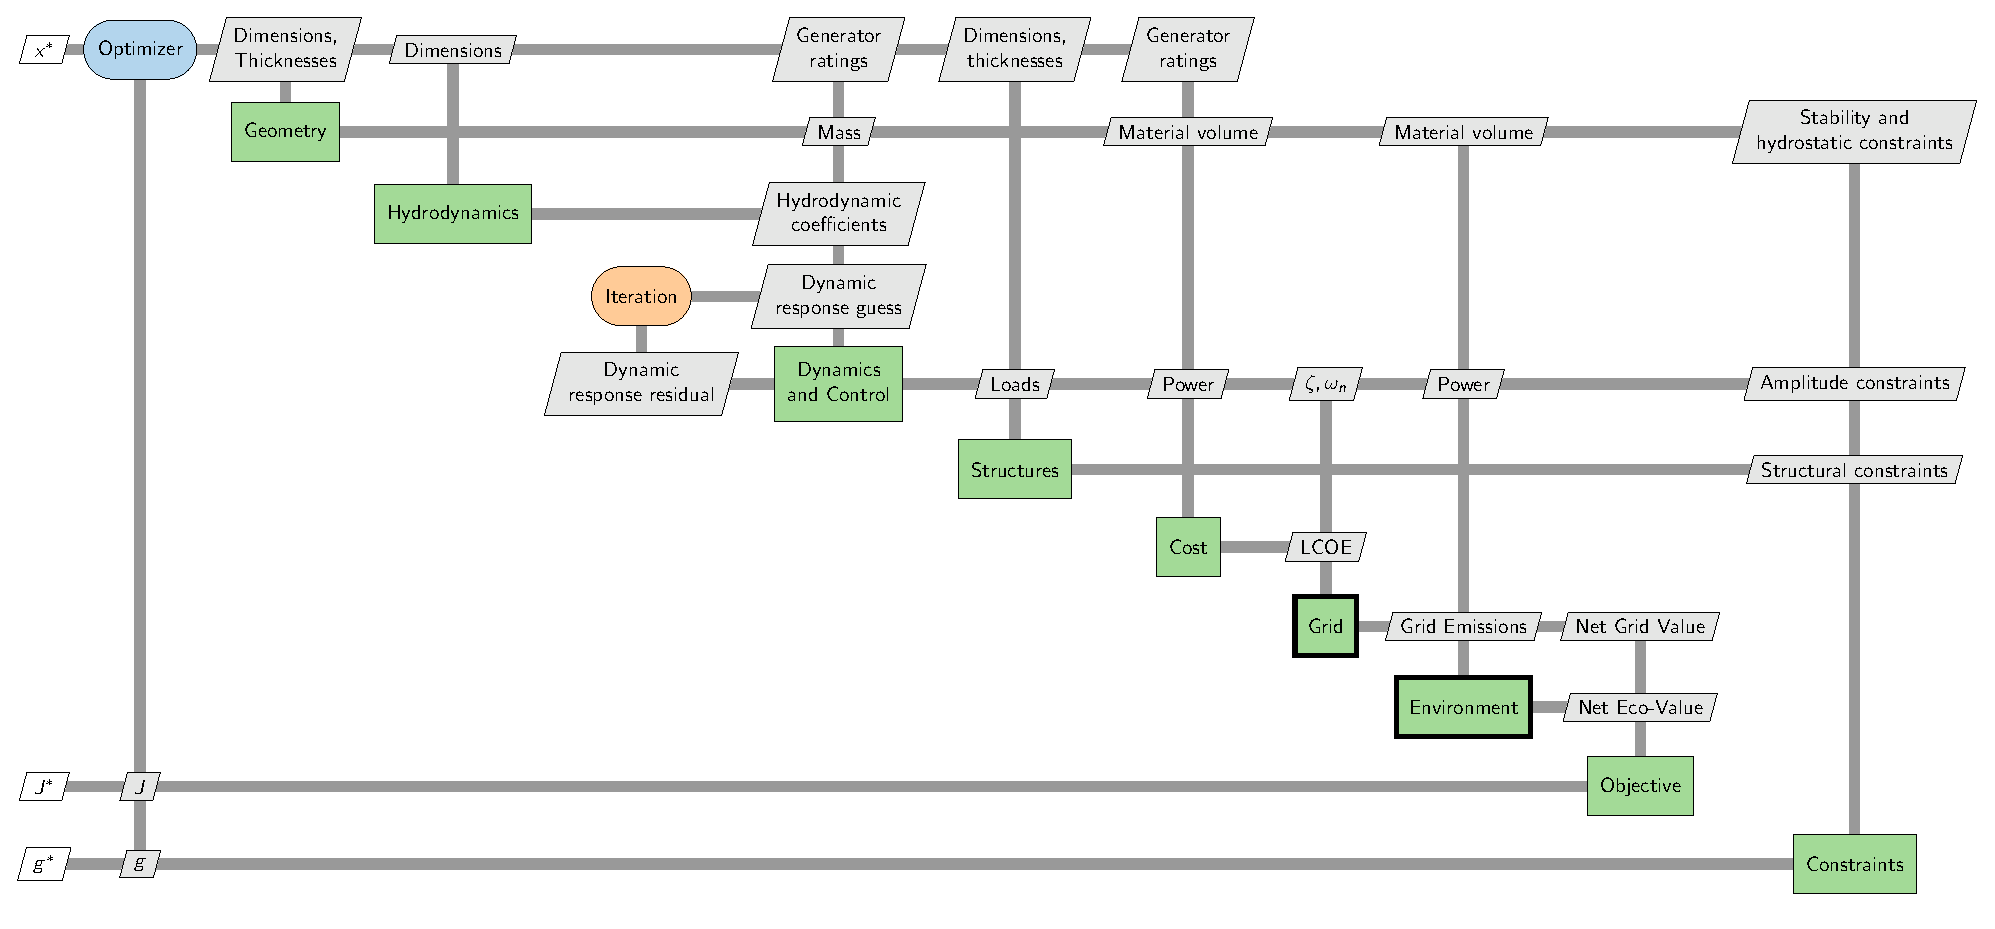
\includegraphics[width=.74\textwidth]{figures/out/xdsm_grid.pdf}
    \caption{xDSM diagram}
    \label{fig:n2}
\end{wrapfigure}


% \begin{wrapfigure}[18]{r}{0.52\textwidth}
%     \centering
%     \includegraphics[width=.5\textwidth]{figures/CEM-flowchart-idetc.png}
%     \caption{Surrogate model diagram}
%     \label{fig:surrogate}
% \end{wrapfigure}

\subsubsection{Capacity expansion model (CEM)}
The GenX CEM \cite{bonaldo_genxprojectgenxjl_2025} is an open-source linear programming model that determines the installed capacity of each generator to minimize the total grid system cost while meeting demand and emissions constraints.
It indirectly enforces economic equilibrium since at the optimum, only generators that cost less than the value they provide are installed.
This implies that NVOE (net value of electricity), a metric which \cite{mowers_evaluation_2021,mccabe_system_2023} suggest using, is always zero in a CEM.
The CEM grid system cost metric captures more effects than NVOE, such as costs and avoided costs of non-WEC generators, storage, and transmission required to balance the grid given the WEC power profile.
%    -  GenX: equation~\eqref{eq:CEM-objective} for the LP it solves
%\begin{equation}\label{eq:CEM-objective}
%    \min_{x_{grid}} C_{grid} = \sum_{gen} \sum_{t} p_{gen,t} x_{grid,gen,t}
%\end{equation}
    %-  time domain reduction and what timescales of power variation and demand alignment are captured vs relevant (seasonality, storms, within wave, within sea state between waves)
    %-  Emissions in CEM
    %-  how we're confident enough that the results aren't due to random chance alignment between that day's demand and wave data and are real / significant
GenX requires as input detailed data on the costs, hourly profiles, and existing infrastructure of all generation, transmission, storage, and load on the grid.
This is managed by the PowerGenome package \cite{schivley_powergenomepowergenome_2025}, which consolidates data from multiple sources such as the U.S. Energy Information Administration (EIA) and National Renewable Energy Laboratory (NREL) including scenarios for reference, moderate, and high levels of electrification.
PowerGenome also allows control over a grid-wide maximum CO\textsubscript{2} constraint.
\figureautorefname~\ref{fig:CEM-data-flow} depicts the data flow for the CEM runs prior to design optimization.
%Coefficients $\beta$ 
Grid costs and emissions are found for each input combination of WEC cost, grid scenario, location, and WEC dynamics (damping ratio and natural frequency).
Orange outlines indicate code implemented in this work rather than an existing package.
PowerGenome does not provide data on wave energy converters, so we use the MHKit interface \cite{klise_mhkit_2020} to NREL hindcast power densities \cite{wu_development_2020,allahdadi_development_2019} along with design-dependent capture width information to generate the hourly power profiles of the WECs. 
Temporal and spatial resolution and scope are set to encompass one year each decade for three decades, with hourly energy profiles, for a northeast and California grid scenario, containing three and two load zones respectively.

\subsubsection{Reduced order model and lookup table}
Linking the design and grid optimization requires first identifying a small number of key design characteristics to collapse the large WEC design space (a reduced order model), and then building a surrogate model to predict the CEM outputs from these reduced design characteristics.
The reduced order model represents the capture width of the WEC, $CW$, as a fraction of the maximum radiative capture width, $CW_{max}=Gg/\omega^2$ \cite{zou_practical_2023}. Physics dictates the following form:
\begin{equation}
    \label{eq:CW-fraction}
    \frac{CW}{CW_{max}} = \frac{2 B_u(\omega) \omega^5}{G \rho g^3} |RAO(\omega)|^2
\end{equation}
with gain $G$ (1 for heave, 2 for surge/pitch), control damping $B_u$, wave energy frequency $\omega$, water density $\rho$, gravitational acceleration $g$, and response amplitude operator $RAO$ (the complex ratio of WEC motion and wave amplitude, $X/\eta$).
%In optimal reactive control, $B_u(\omega)=B_h(\omega)+B_d(\omega,RAO(\omega))$, where $B_h$ is the hydrodynamic damping and $B_d$ is nonlinear drag damping. 
We assume the RAO is a standard second order system with damping ratio $\zeta$ and natural frequency $\omega_n$ \cite{franklin2014feedback}:
\begin{equation}
    \label{eq:rao}
    RAO(\omega) = \frac{1}{1-\left(\frac{\omega}{\omega_n}\right)^2 + j 2 \zeta \frac{\omega}{\omega_n}}
\end{equation}
with imaginary unit $j$.
This second-order assumption implies $\Im(RAO)=2\zeta \omega_n$.
If combined with the optimal reactive control law $B_u(\omega) = \Im(RAO(\omega))/2$, this forces a frequency-independent control damping.
The values of $\zeta$ and $\omega_n$ for a given design are determined via a least-squares fit of the dynamics module output to equation \eqref{eq:rao} across all sea states with nonzero probability in the JPD.
Using frequency index $i$ and wave height index $j$, this is expressed:
%(equation~\eqref{eq:bode-fit}),
%\begin{equation}
%\begin{aligned}
%    \zeta,\omega_n &= \mathrm{argmin}\left( \epsilon_{mag}^2 + \epsilon_{phase}^2 \right) \\
%    \epsilon_{mag} &= xxx \\
%    \epsilon_{phase} &= xxx
%\end{aligned}
%\end{equation}
\begin{equation}\label{eq:bode-fit}
    \zeta,\omega_n = \mathrm{argmin}(\epsilon_{mag}^2), \quad
    \epsilon_{mag} = \sum_{i,j}^{} \left(\left|\frac{X_{ij}}{\eta_j}\right|-\left|\frac{1}{1-\left(\frac{\omega_i}{\omega_n}\right)^2 + j 2 \zeta \frac{\omega_i}{\omega_n}}\right|\right)
\end{equation}
For RM3, this model is found to be valid at frequencies at and below resonance, shown in \figureautorefname~\ref{fig:bode}.
Capturing the behavior above resonance would require a higher order model such as one with five poles, two standard zeros, and two right half plane zeros.
However, sweeping 9 dynamic inputs to the CEM instead of 2 would be computationally costly, and high frequencies are less common in the ocean, so this study maintains a second order model.
Future work could also incorporate drag nonlinearities by allowing $\zeta$ to vary with wave height.
The reduced order model is used only to capture the effect of WEC design on the hourly variability profile input to the CEM, not to calculate energy production.

    %- assumes that the WEC can generate less than its max power without violating any amplitude/force constraints        
    %-  how CEM system cost gets turned into NVOE metric (since CEM enforces NVOE=0)    

Meanwhile, the surrogate model is in this case simply a lookup table with linear interpolation.
Future work could develop a more mechanistic surrogate model to understand driving factors and allow extrapolation to different grid scenarios.
The use of the surrogate model makes the computational cost low enough to allow the design optimization to utilize the CEM outputs.
This approach accurately takes into account marginal generators, unlike wind turbine studies \cite{canet_eco-conscious_2023,kainz_technological_2024} which correlate historical spot market price and grid emissions with wind speed, location, and hub height rather than using a CEM.
%In addition to the directly used CEM outputs of grid cost and emissions, we use additional CEM outputs (installed capacity of WECs and other generators) and compute indirect CEM outputs (maximum cost threshold) as part of the surrogate model to predict the primary outputs from design inputs. 
%The maximum threshold cost represents the maximum cost of any generator (with the most favorable generation profile) that would be installed for each grid scenario.

\begin{figure}[b]
\noindent
\begin{minipage}[t]{0.32\textwidth}
    \centering
    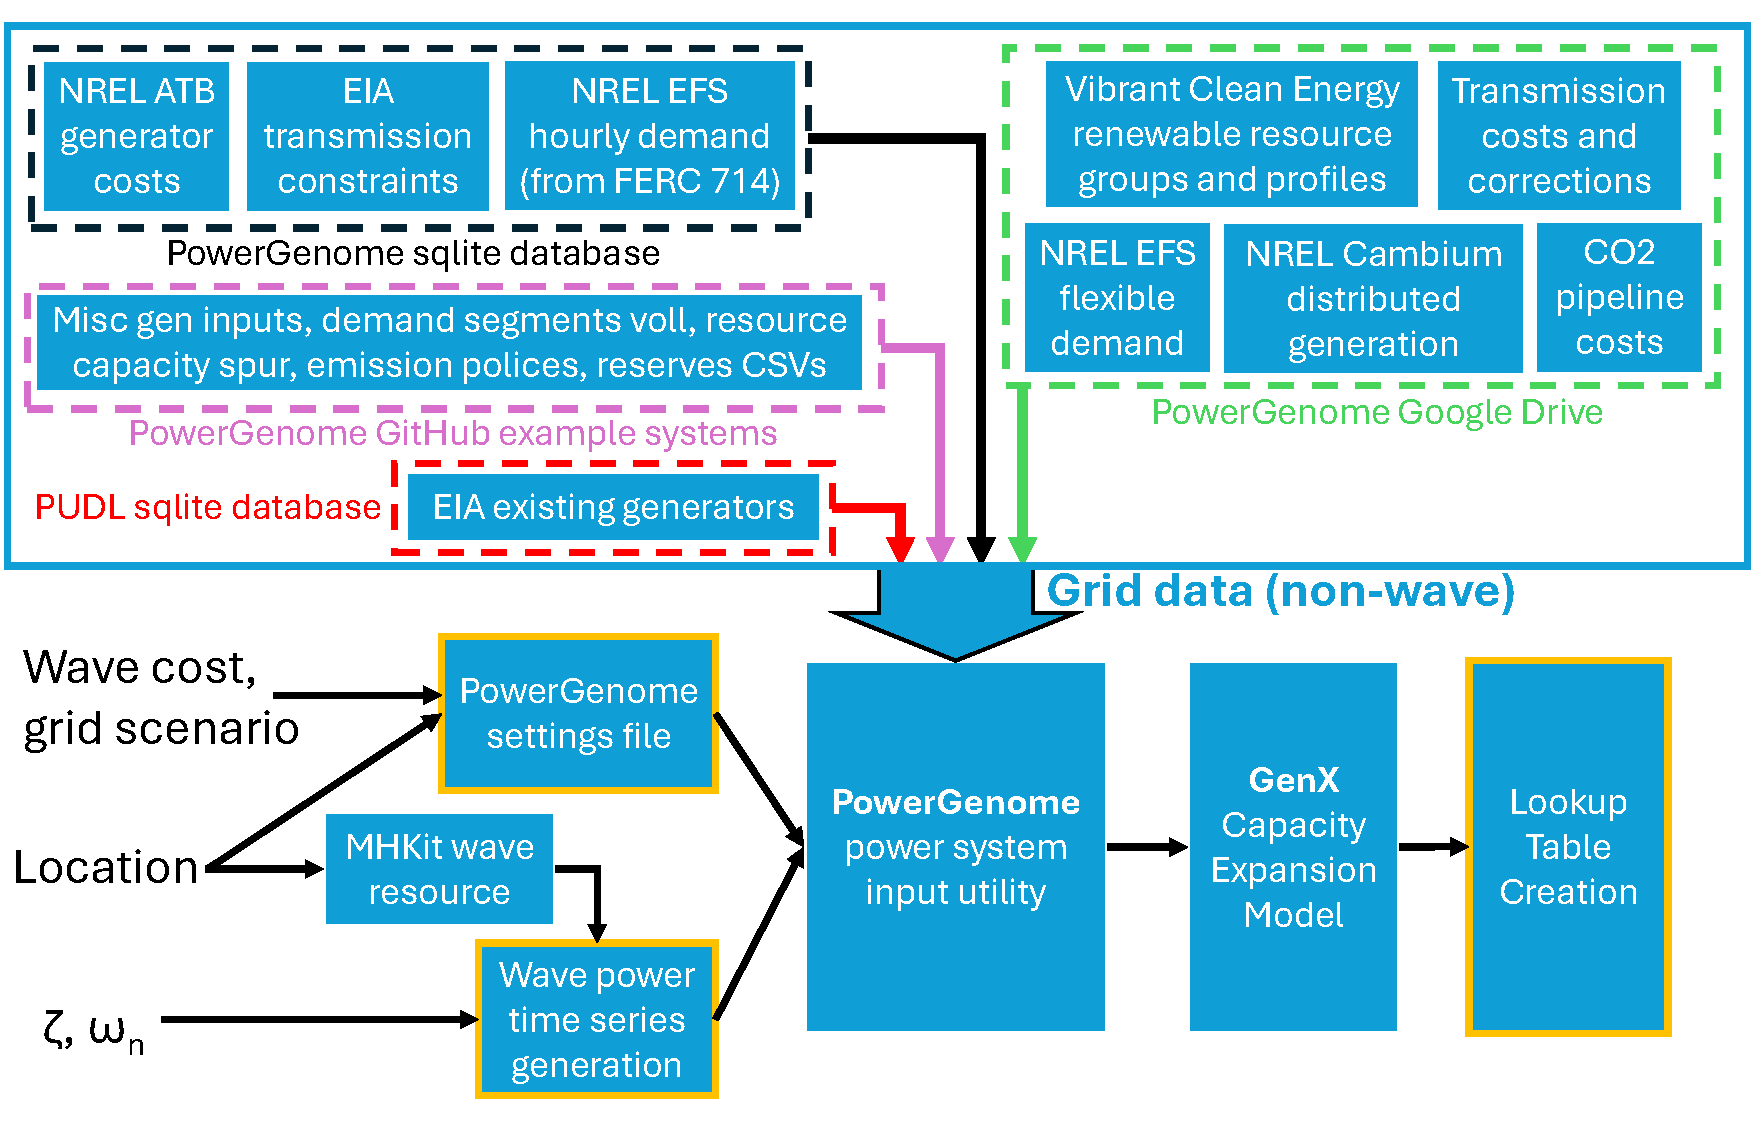
\includegraphics[width=\linewidth]{figures/PowerGenomeDataFlow_no_beta.pdf}
    \captionof{figure}{Data flow for the CEM}
    \label{fig:CEM-data-flow}
\end{minipage}
\hfill
\begin{minipage}[t]{0.32\textwidth}
    \centering
    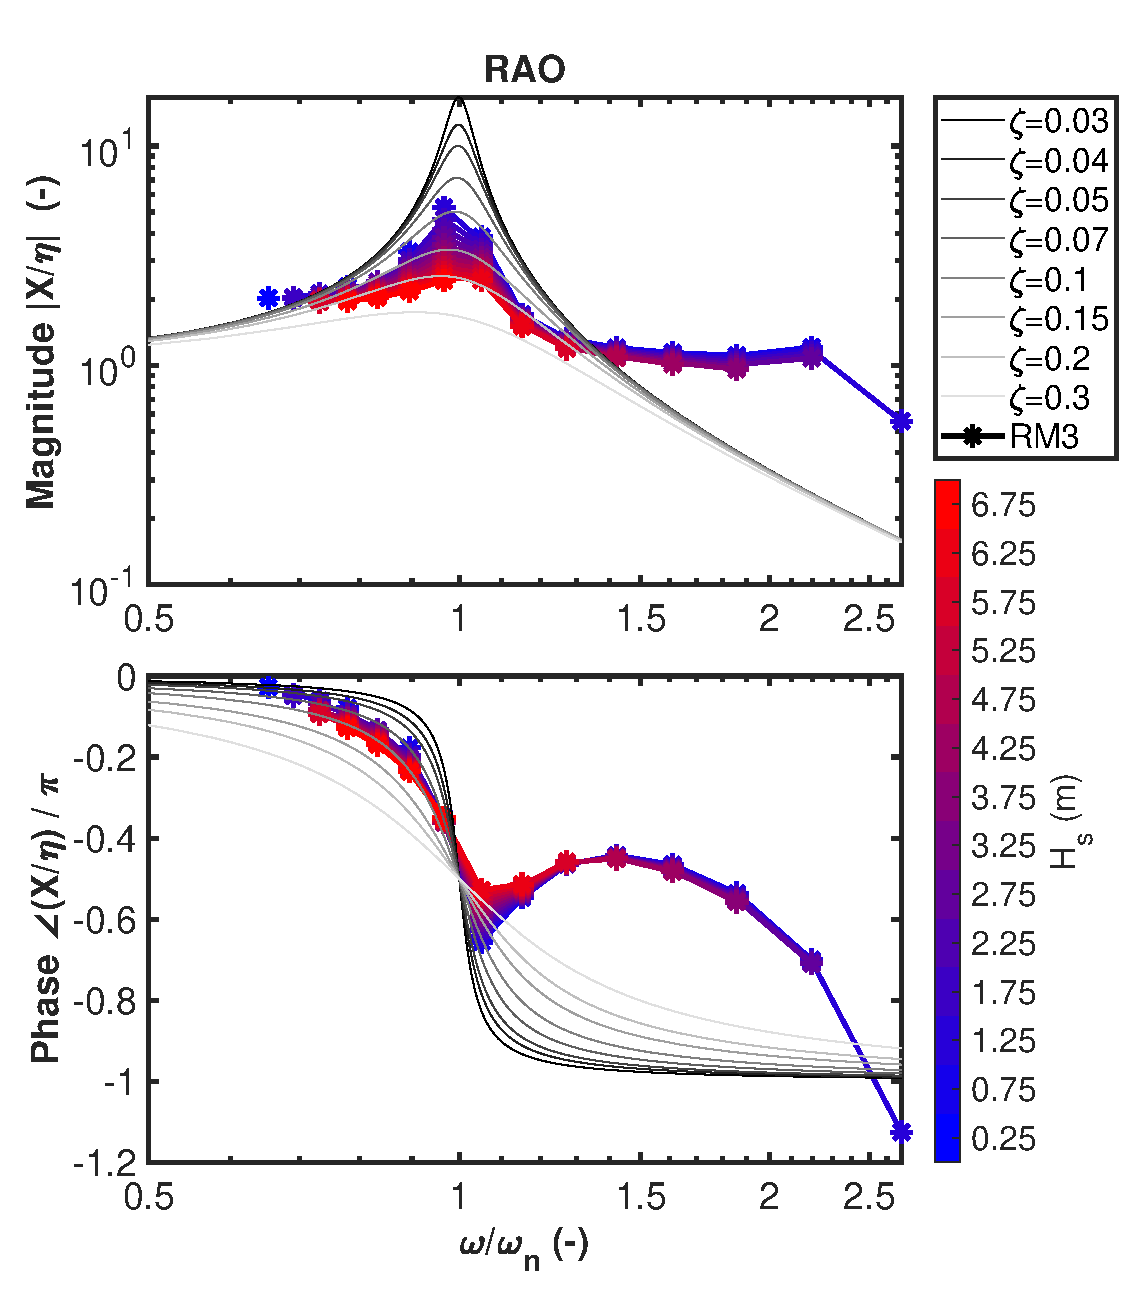
\includegraphics[width=\linewidth]{figures/bode_second_order.pdf}
    \captionof{figure}{Bode fit}
    \label{fig:bode}
\end{minipage}
\hfill
\begin{minipage}[t]{0.32\textwidth}
    \centering
    \includegraphics[width=\linewidth]{example-image-a}
    \captionof{figure}{CEM output raw data and fit}
    \label{fig:three}
\end{minipage}
\end{figure}

\subsubsection{Life cycle analysis (LCA)}
LCA in the early design phase is challenging due to uncertainties in materials, manufacturing, and transportation.
Fortunately, optimization only requires modeling effects that meaningfully scale with design variables.
This includes material use (steel, fiberglass) but not aquatic habitat disruption or hydraulic fluid toxicity since they are not captured in MDOcean's low design fidelity.
Although the present study holds distance from shore constant, the environmental model includes offshore transportation (diesel fuel) so future work can evaluate the tradeoff between better energetics but worse survivability, operating cost, and maintenance emissions for WECs further offshore.

MDOcean calculates WEC structural material masses in the MDOcean geometry module and multiplies them by appropriate weighting coefficients in the environment module.
We utilize the Idemat LCA dataset \cite{idemat}, which provides a set of eco-cost coefficients \cite{vogtlander_lca-based_2010} that express the lifetime environmental impacts of various materials and processes across diverse axes (i.e. water, emissions, pollution) in monetary units (see \tableautorefname~\ref{tab:lca-weights}).
MDOcean then offsets the eco-cost with the eco-value of CEM avoided grid emissions using the social cost of carbon, and finally normalizes by CEM WEC grid energy production to obtain the net eco-value per unit energy (\$/kWh).

Inspecting the model reveals three takeaways.
First, the eco-cost computed here represents only around XX\% of the eco-cost of prior WEC LCA studies \cite{LCA}, indicating that most of the eco-cost (is/is not) cemented (before/until) the detail design phase.
Second, the eco-value far exceeds the eco-cost, indicating that LCA-informed environmental optimization to reduce eco-cost will be less relevant than economic optimization to enable WECs to displace fossil fuel generators.
Third, the eco-cost coefficients for steel and fiberglass are similar to their economic prices, indicating that the economic-optimal and environmental-optimal designs are expected to be similar.
% show this with numbers
All three of these observations imply that design-for-environment techniques have limited utility at the early design stage, although the multi-objective optimization is still performed to confirm these conclusions.

\begin{table}[H]
    \begin{center}
    \caption{Eco-cost coefficients}
    \begin{tabular}{ lll } 
     \hline
     Material/component & Value & Unit \\ 
     \hline
     Steel & xx & \$/kg \\ 
     Fiberglass & xx & \$/m\textsuperscript{2} \\ 
     Distance from shore & xx & \$/km \\ 
     Social cost of carbon & xx & \$/tCO\textsubscript{2,e} \\
    \end{tabular}
    
    \label{tab:lca-weights}
    \end{center}
\end{table}


\section{Results}
    -  CEM sweep (no optim) raw vs fitted
    -  single obj optim (min NVOE compared to min LCOE)
    -  multi obj optim (pareto NVOE vs net eco value per power)
    -  runtime info
    -  when WECs are viable, what are they replacing (batteries or wind or solar etc)? Find by looking at how does the optimal LP output change with
    -  can the CEM results be predicted by correlation coefficient of WEC power with demand or with energy storage or with lost load of solar, the capacity factor, sum of hourly profit, other proxies?

    Enviro not being a big deal: While this study hypothesized the opposite, hoping to quantify an economic-environmental tradeoff, the exercise of building the model suggests that economic and environmental objectives align in the early design phase.
and that environmentally-conscious engineers can feel satisfied that economic optimization also benefits the environmental bottom line.

\begin{figure}[b]
\noindent
\begin{minipage}[t]{0.32\textwidth}
    \centering
    \includegraphics[width=\linewidth]{example-image-a}
    \captionof{figure}{CEM results: beta and confidence bounds for various grid scenarios}
    \label{fig:cem-results}
\end{minipage}
\hfill
\begin{minipage}[t]{0.32\textwidth}
    \centering
    \includegraphics[width=\linewidth]{example-image-a}
    \captionof{figure}{Comparison of single-objective optima}
    \label{fig:single-obj-compare}
\end{minipage}
\hfill
\begin{minipage}[t]{0.32\textwidth}
    \centering
    \includegraphics[width=\linewidth]{example-image-a}
    \captionof{figure}{Pareto front}
    \label{fig:pareto}
\end{minipage}
\end{figure}

\lipsum[1-3]

\section{Conclusions}
\lipsum[1]

- do we see WECs being viable NVOE-wise despite a high LCOE due to their temporal

- does optimizing for NVOE vs LCOE make a big difference in the optimal design?

\section*{Acknowledgments and Data Availability}
%%%%%%%%%%%%%%%%%%%%%%%%%%%%%%%%%%%%%%%%%%%%%%%%%%%%%%%%%%%%%%%%%%%%%%%%%%%%%%%%%%%%%%%%%%%%%%%%%%%%%%%%
The authors thank Olivia Vitale and Collin Treacy for feedback on a draft manuscript. Code to fully reproduce this work is available open-source: design optimization at \url{github.com/symbiotic-engineering/MDOcean} and capacity expansion model at \url{github.com/symbiotic-engineering/wec-decider}.

\clearpage
\section{Main Text}

\begin{framed}
\textbf{Nomenclature} \\
\normalsize    
    A\ \ \ \ radius of \\    
    B \ \ \ \ position of \\    
    C\ \ \ \ further nomenclature continues down the page inside the text box \\
\end{framed}


%------------------------------------------------------------------------------------------------------%
\subsection{Tables}
%------------------------------------------------------------------------------------------------------%
Headings should be placed above tables, left justified. Only horizontal lines should be used within a table, to distinguish the column headings from the body of the table, and immediately above and below the table.

%------------------------------------------------------------------------------------------------------%
\subsection{Section headings}
%------------------------------------------------------------------------------------------------------%
Sub-section headings should be bold, in capital and lower-case italic letters, numbered 1.1, 1.2, etc., and left justified, with second and subsequent lines indented. 

%------------------------------------------------------------------------------------------------------%
\subsection{Footnotes}
%------------------------------------------------------------------------------------------------------%
Footnotes should be avoided if possible. Necessary footnotes should be denoted in the text by consecutive superscript letters\footnote{1 Footnote text.} \cite{mccabe_system_2023,mccabe_mdocean_2024}. The footnotes should be typed single spaced, and in smaller type size (8 pt), at the foot of the page in which they are mentioned, and separated from the main text by a one line space extending at the foot of the column.

%------------------------------------------------------------------------------------------------------%
\section{Illustrations}
%------------------------------------------------------------------------------------------------------%
Figures should be placed at the top or bottom of a page wherever possible, as close as possible to the first reference to them in the paper. The figure number and caption should be typed below the illustration in 8 pt and centered with the image. If two images fit next to each other, these may be placed next to each other to save space.


%%%%%%%%%%%%%%%%%%%%%%%%%%%%%%%%%%%%%%%%%%%%%%%%%%%%%%%%%%%%%%%%%%%%%%%%%%%%%%%%%%%%%%%%%%%%%%%%%%%%%%%%

%%%%%%%%%%%%%%%%%%%%%%%%%%%%%%%%%%%%%%%%%%%%%%%%%%%%%%%%%%%%%%%%%%%%%%%%%%%%%%%%%%%%%%%%%%%%%%%%%%%%%%%%


\vspace{1\baselineskip}

%%%%%%%%%%%%%%%%%%%%%%%%%%%%%%%%%%%%%%%%%%%%%%%%%%%%%%%%%%%%%%%%%%%%%%%%%%%%%%%%%%%%%%%%%%%%%%%%%%%%%%%%
\section*{Appendix A. CEM Surrogate model equation}
%%%%%%%%%%%%%%%%%%%%%%%%%%%%%%%%%%%%%%%%%%%%%%%%%%%%%%%%%%%%%%%%%%%%%%%%%%%%%%%%%%%%%%%%%%%%%%%%%%%%%%%%
$C$ refers to costs (\$M) (output from CEM), $S$ refers to specific capacity costs (\$M/kW) (input to CEM), $x_{grid}$ refers to installed capacities (decision variable in CEM), and $E$ refers to specific energy costs (\$/kWh). The amount of built wave capacity $x_{grid,WEC}$ is not to be confused with $x_{design}$, the WEC design variables in the outer (MDOcean) optimization that are parameters (held constant) in the CEM.

\begin{equation}
\begin{aligned}
    C_{grid}(p_{grid},x_{design}) &= C_{grid,0}(p_{grid})- \beta_1(p_{grid})~ x_{grid,WEC}(p_{grid},x_{design}) \\
    \frac{x_{grid,WEC}(p_{grid},x_{design})}{x_{grid,WEC}(p_{grid},x_{design})+\sum_{gen\neq WEC}x_{grid,gen}(p_{grid},x_{design})} &= \min\left(\beta_2(p_{grid}) \times \max\left(\frac{S_{WEC,thresh}(p_{grid},x_{design})}{S_{WEC}(x_{design})}-1,0\right), 1\right) \\
    S_{WEC,thresh}(p_{grid},x_{design}) &= S_{max,thresh}(p_{grid}) - \beta_3(p_{grid}) \zeta(x_{design}) - \beta_4(p_{grid}) \frac{\omega_n}{\omega_p}(x_{design}) - \beta_5(p_{grid}) \min\left(\frac{P_{max}}{P_{pk}}(x_{design}),1\right) \\
    \sum_{gen\neq WEC}x_{grid,gen}(p_{grid},x_{design}) &= \sum_{gen}x_{grid,gen,0}(p_{grid})-\beta_6(p_{grid}) \zeta(x_{design}) - \beta_7(p_{grid}) \frac{\omega_n}{\omega_p}(x_{design}) - \beta_8(p_{grid}) \min\left(\frac{P_{max}}{P_{pk}}(x_{design}),1\right)
\end{aligned}
\end{equation}

%improvements to make to above eqn:
%- debatable whether coeffs should be kept dimensional, ie should $\beta_1$ get divided by total capacity and $C_{grid,0}(p_{grid})$ so it's relating percent cost to percent capacity?
%- $\beta_{3-8}$ terms could be made nonlinear as needed - ie $(\frac{\omega_n}{\omega_p})^2-1$ shows up in theory. I could also try to feed-forward incorporate the time domain power reconstruction, ie a peak to average ratio, if that is looking like a better fit than the freq domain stuff, but that just tells me that my hope of doing freq domain to connect to mdocean won't work out.
%- ideally some of these betas turn out to be independent of p grid, which means more of the p grid dependence can be found just from the 0 (no wec) case for that p, without requiring a whole design sweep. That is the reason all this modeling is potentially more useful than a lookup table.
%- Could add saturation to make sure $S_{WEC,thresh}>0$ and $C_{grid}>0$.
%- add hats or some other notation to differentiate predicted (fit) from actual

\vspace{1\baselineskip}
\textit{A.1 Example of a sub-heading within an appendix}
\vspace{1\baselineskip}

There is also the option to include a subheading within the Appendix if you wish.

%%%%%%%%%%%%%%%%%%%%%%%%%%%%%%%%%%%%%%%%%%%%%%%%%%%%%%%%%%%%%%%%%%%%%%%%%%%%%%%%%%%%%%%%%%%%%%%%%%%%%%%%% References
%%%%%%%%%%%%%%%%%%%%%%%%%%%%%%%%%%%%%%%%%%%%%%%%%%%%%%%%%%%%%%%%%%%%%%%%%%%%%%%%%%%%%%%%%%%%%%%%%%%%%%%%

\printbibliography

\end{document}